\section{Regularization for Deep Learning}
\begin{multicols}{2}
	A goal of machine learning is, that the algorithm generalizes, that is, that it will perform well on data it has never been trained with.
	Regularization is any strategy that is designed to reduce the test error, often at the expense of increasing the training error.

	\subsection{Parameter Norm Penalties}
	Many regularization approaches are based on limiting the capacity of models by adding a parameter norm penalty to the objective function as
	\[ \tilde{J}(\bolt;\mX,\vy) = J(\bolt;\mX,\vy)+\alpha\Omega(\bolt) \]
	Here $\alpha$ is a nonnegative hyperparameter that weights the contribution of the norm penalty.\\

	Note that in deep learning, the biases (which are part of the parameter set) are usually not part of the norm penalty, since this can introduce a significant amount of underfitting. Hence only the weight matrices are usually regularized using a norm penalty. So instead of using $\bolt$, the vector $\vw$ (containing all the weights) is now used in the norm penalty function.

	\subsection{$L^2$ Parameter Regularization}
	When the Euclidean norm is used for the penalty, than a scheme called weight decay results.
	Note this scheme is also called ridge regression or Tikhonov regularization.
	\[ \Omega(\bolt) = \frac{1}{2} \lVert \vw \rVert_2^2 \]

	It is now clear what happens at a single step, the weights decay towards zero:
	\[ \vw \leftarrow (1-\epsilon\alpha)\vw-\epsilon\nabla_\vw J(\vw;\mX,\vy) \]

	A quadratic approximation to the unregularized objective function $J$ in the neighborhood of the value of the weights $\vw^\ast$ that obtains minimal unregularized cost $J$ is employed
	\[ \vw^\ast = \argmin_\vw J(\vw) \]

	This approximation is given by the expression
	\[ \hat{J}(\bolt) = J(\vw^\ast)+\half(\vw-\vw^\ast)^T\mH(\vw-\vw^\ast) \]
	$\mH$ is the Hessian of $J$ with respect to $\vw$ evaluated at $\vw^\ast$, and is positive semidefinite.
	Clearly the minimum of this approximation occurs where its gradient is zero (since this is a quadratic function), which is at $\vw^\ast$
	\[ \nabla_\vw \hat{J}(\vw)=\mH(\vw-\vw^\ast) \]

	Now the weight decay gradient is added to the gradient of the unregularized cost $J$, resulting in the gradient of the regularized cost and setting it to zero to find the minimum $\tilde{\vw}$ of the regularized cost.
	\begin{align*}
	\nabla_\vw \tilde{J}(\vw;\mX,\vy)
	&= \alpha\vw + \overbrace{\nabla_\vw J(\vw;\mX,\vy)}^{\nabla_\vw\hat{J}(\vw)=\mH(\vw-\vw^\ast)}\\
	\alpha\tilde{\vw}+\mH(\tilde{\vw}-\vw^\ast) &= 0\\
	(\mH+\alpha\mI)\tilde{\vw} &= \mH\vw^\ast\\
	\tilde{\vw}&=(\mH+\alpha\mI)^{-1}\mH\vw^\ast
	\end{align*}
	The final line shows, that if $\alpha$ approaches zero, the regularized solution $\tilde{\vw}$ approaches $\vw^\ast$, the unregularized minimum.\\
	What happens if $\alpha$ grows? Since $\mH$ is real and symmetric, it can be decomposed into a diagonal matrix and an orthonormal basis of eigenvectors as
	\[ \mH = \mQ\bol{\Lambda}\mQ^T \]

	Hence we can apply this decomposition and the following equation results
	\begin{align*}
	\tilde{\vw}	&= (\mH+\alpha\mI)^{-1}\mH\vw^\ast\\
	&= (\mQ\bol{\Lambda}\mQ^T+\alpha\mI)^{-1}\mQ\bol{\Lambda}\mQ^T\vw^\ast\\
	&=\left[\mQ(\bol{\Lambda}+\alpha\mI)\mQ^T\right]^{-1}\mQ\bol{\Lambda}\mQ^T\vw^\ast\\
	&= \mQ(\bol{\Lambda}+\alpha\mI)^{-1}\bol{\Lambda}\mQ^T\vw^\ast
	\end{align*}
	Multiplying from the left with $\mQ^T$ results in the following relationship between $\mQ^T\tilde{\vw}$ and $\mQ^T\vw^\ast$:
	\[ \left[\mQ^T\tilde{\vw}\right] =(\bol{\Lambda}+\alpha\mI)^{-1}\bol{\Lambda}\left[\mQ^T\vw^\ast\right] \]
	Consider the vector $\left[\mQ^T\vw^\ast\right]$, which is $\vw^\ast$ expressed in terms of the eigenvectors.\\
	Consider the vector $\left[\mQ^T\tilde{\vw}\right]$, which is $\tilde{\vw}$ expressed in terms of the eigenvectors.\\
	The matrix $(\bol{\Lambda}+\alpha\mI)^{-1}\bol{\Lambda}$ is a diagonal matrix with the diagonal elements
	\[ \frac{\lambda_i}{\lambda_i+\alpha} \]
	Hence, the component of $\vw^\ast$ that is aligned with the $i^{\text{th}}$ eigenvector of $\mH$ is rescaled by the factor $\lambda_i/(\lambda_i+\alpha)$.\\

	Along the directions where the eigenvalues of $\mH$ are relatively large, the effect of regularization is relatively small.
	However, components with small $\lambda$s, will be shrunk to have nearly zero magnitude.
	Only directions along which the parameters contribute significantly to reducing the unregularized $J$ are preserved relatively intact. In directions that do not contribute to reducing the unregularized $J$, a small eigenvalue of the Hessian tells us that movement in this direction will not significantly increase the gradient.\\

	Now this analysis is applied to linear regression.
	Note that in linear regression, the true cost function is quadratic and hence the approximation used so far fits the model perfectly
	\[ \hat{y} = \mX\vw \]
	The corresponding optimal solution is
	\[ \vw = (\mX^T\mX)^{-1}\mX^T\vy \]
	Now the $L^2$ regularization term is added, resulting in the new objective function
	\[ (\mX\vw-\vy)^T(\mX\vw-\vy)+\half\alpha\vw^T\vw \]
	and the corresponding optimal solution is
	\[ \vw = (\mX^T\mX+\alpha\mI)^{-1}\mX^T\vy \]
	Note that $\mX^T\mX$ is proportional to the covariance matrix $(\mX^T\mX)/m$.
	$L^2$ regularization replaces $\mX^T\mX$ with $(\mX^T\mX+\alpha\mI)$, hence the same matrix but with an additional $\alpha$ term added to the diagonal elements.

	\subsection{$L^1$ Regularization}
	An alternative is $L^1$ regularization where the penalty term is defined as
	\[ \Omega(\bolt) = \lVert\vw\rVert_1 = \sum_i \lvert w_i\rvert \]

	The regularized objective function now becomes
	\[ \tilde{J}(\vw;\mX,\vy) = \alpha\lVert\vw\rVert_1+j(\vw;\mX,\vy) \]

	This results in the following gradient w.r.t. the weights $\vw$
	\[ \nabla_\vw \tilde{J}(\vw;\mX,\vy)=\alpha \sign(\vw)+\nabla_\vw J(\mX,\vy;\vw) \]
	Note the sign function is applied elementwise, i.e., results in a vector filled with +1 or -1.\\
	$L^1$ regularization is clearly quite different. The contribution of the regularization to the gradient no longer scales linearly with each $w_i$, instead it is a constant factor $\alpha$ with the sign equal to the sign of $w_i$.\\

	The problem of minimizing this approximate cost function has an analytical solution (for each dimension $i$), with the following form:
	\begin{align*}
	\tilde{\hat{J}}(\vw;\mX,\vy)
	&= J(\vw^\ast;\mX,\vy)+\sum_i\left[\half H_{i,i}(\vw_i-\vw_i^\ast)^2+\alpha\lvert w_i\rvert\right]\\
	w_i &= \sign(w_i^\ast)\max\left\{ \lvert w_i^\ast\rvert-\frac{\alpha}{H_{i,i}},0 \right\}
	\end{align*}

	The graph below shows that $L^1$ results in more zero weights than $L^2$, hence $L^1$ regularization results in a sparser solution. $L^2$ does not encourage zero explicitly but only favors smaller values.
	\begin{figure}[H]
		\centering
		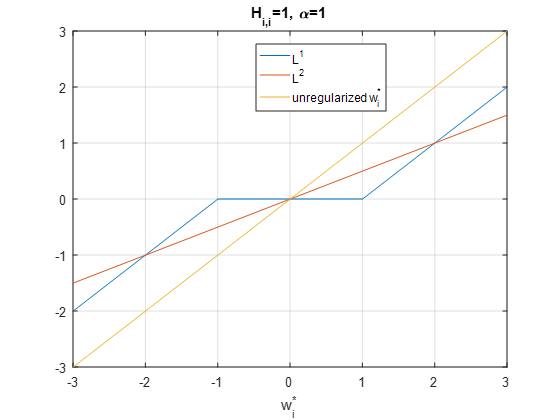
\includegraphics[width=0.9\linewidth]{images/L1L2.png}
	\end{figure}

	\subsection{Early Stopping}
	When the model has sufficient capacity to overfit, then the learning curves should look like the one below:
	\begin{figure}[H]
		\centering
		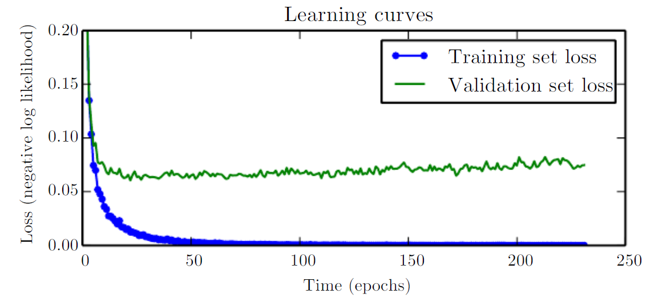
\includegraphics[width=0.9\linewidth]{images/earlystopping.png}
	\end{figure}
	Hence the model after 200 epochs is worse at the validation data set than after 30 epochs, so the model at 30 epochs should be used, since a better validation error should also result in a better test error.\\

	Early stopping is an unobtrusive form of regularization, in that it requires almost no change in the underlying training procedure, the objective function, or the set of allowable parameter values.
	This means that it is easy to use early stopping without damaging the learning dynamics.
	This is \textbf{in contrast to weight decay}, where one must be careful not to use too much weight decay and trap the network in a bad local minimum corresponding to a solution with pathologically small weights.\\

	Early stopping requires a validation set, hence some labeled data is not used for training.
	There are three basic approaches how this data can be used for training the model:
	\begin{enumerate}
		\item Don’t do it, just have enough data
		\item Expensive idea: once early stopping has figured out the optimal number of training epochs, reset everything and train for this optimal number of iterations using all data
		\begin{itemize}
			\item[$\rightarrow$] Usually not done in practice, where the training sets are large and the training takes a long time
		\end{itemize}
		\item Less expensive idea, but a bit tricky: Basically after the stopping criterion has been reached, keep training, now using all the data
	\end{enumerate}
	How does early stopping act as a regularizer?\\
	\vdots\\
	Under the given assumptions, the number of training iterations $\tau$ plays a role inversely proportional to the $L^2$ regularization parameter $\alpha$:
	\[ \alpha \approx \frac{1}{\tau\epsilon} \]
	\begin{figure}[H]
		\centering
		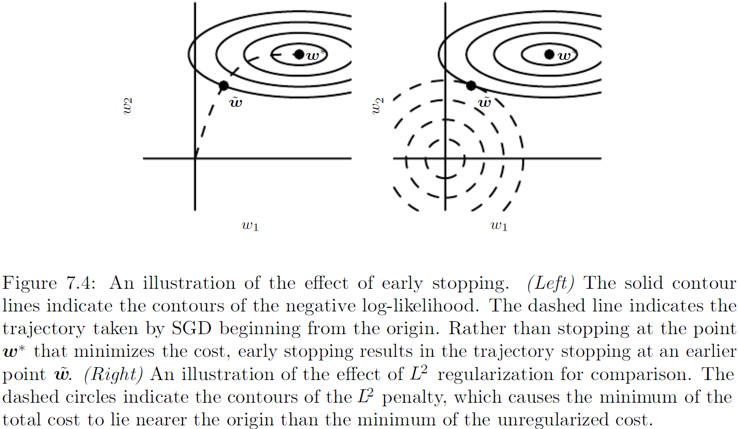
\includegraphics[width=1\linewidth]{images/earlyvsl2.png}
	\end{figure}
	As we have shown before, parameter values corresponding to directions of significant curvature (of the objective function) are regularized less than directions of less curvature. Of course, in the context of early stopping, this really means that parameters that correspond to directions of significant curvature tend to be learned \textbf{early} relative to parameters corresponding to directions of less curvature.
		\subsection{Dataset Augmentation}
	The best way to make a machine learning model generalize better, is to train it on more data. Dataset augmentation is directly applicable for classification, where a mapping between some high dimensional input \textbf{x} and a single category y needs to be learned.
	A few approaches for object recognition:
	\begin{itemize}
		\item Random Cropping
		\item Random color shift
		\item Noise injection
	\end{itemize}
	Dataset Augementation has also been very successful in speech recognition.
	\begin{figure}[H]
		\centering
		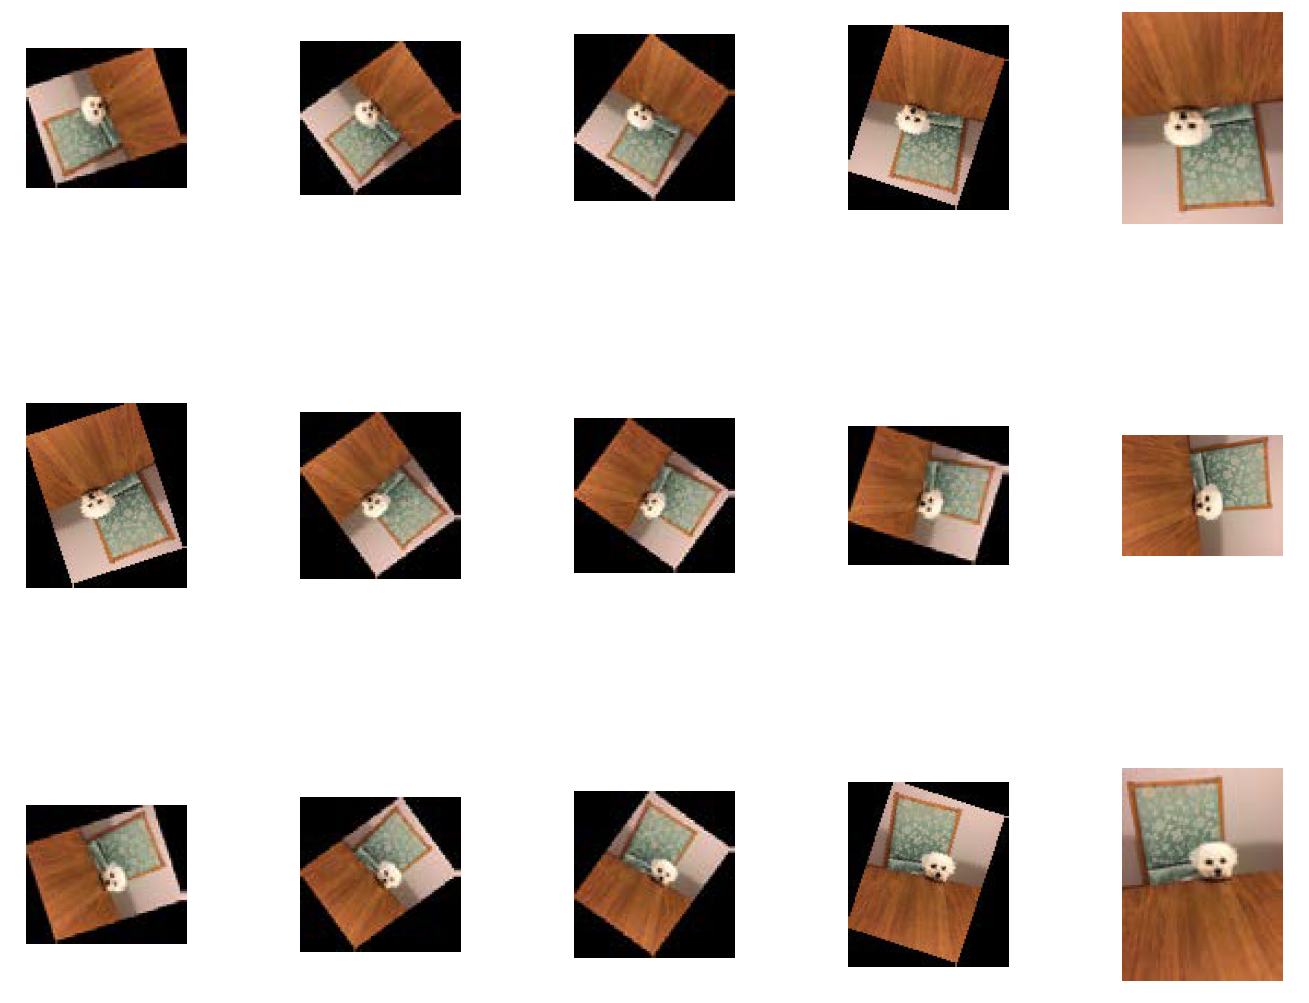
\includegraphics[width=1\linewidth]{images/datasetAugementation.PNG}
	\end{figure}

	\subsection{Bagging and other Ensemble Methods}
	The idea is to train several different models separately, then have all of the models vote on the output for test examples.
	This is an example of a general strategy in machine learning called model averaging. Techniques employing this strategy are known as \textbf{ensemble methods}.
	The main reason why this works is, that different models will make different, and \emph{ideally, uncorrelated}, errors. Hence averaging the model responses will reduce the variance of the errors:
	\begin{align*}
	\E\left[\left(\frac{1}{k}\sum_i\epsilon_i\right)^2\right]
	&= \frac{1}{k^2}\E\left[\sum_i\left(\epsilon_i^2+\sum_{j\neq i}\epsilon_i\epsilon_j\right)\right]\\
	&= \frac{1}{k}v+\frac{k-1}{k}c
	\end{align*}
	The formula clearly shows, that for perfectly correlated errors $(c=v)$, averaging the predictions and hence averaging the errors does not help.
	In the case the errors are completely \textbf{uncorrelated} $c=0$, the well known result is achieved, that the error variance $v$ is reduced by the number of models $k$.
	Hence in the \textbf{worst case} it is not worse than a single model.
	In the \textbf{best case} it is better by a factor $k$. This assumes that the mean error is zero.\\

	\textbf{Bootstrap aggregating (bagging)} is a method that allows the same kind of model, training algorithm and objective function to be reused several times.
	Bagging involves constructing $k$ different datasets. Each dataset has the same number of examples as the original dataset, but each dataset is constructed by sampling with replacement from the original dataset.\\
	This means that, with high probability, each dataset is missing some of the examples from the original dataset and also contains several duplicate examples (on average around $2/3$ of the examples from the original dataset are found in the resulting training set, if it has the same size as the original).\\
	Model $i$ is then trained on dataset $i$. The differences between which examples are included in each dataset result in differences between the trained models.
	\begin{figure}[H]
		\centering
		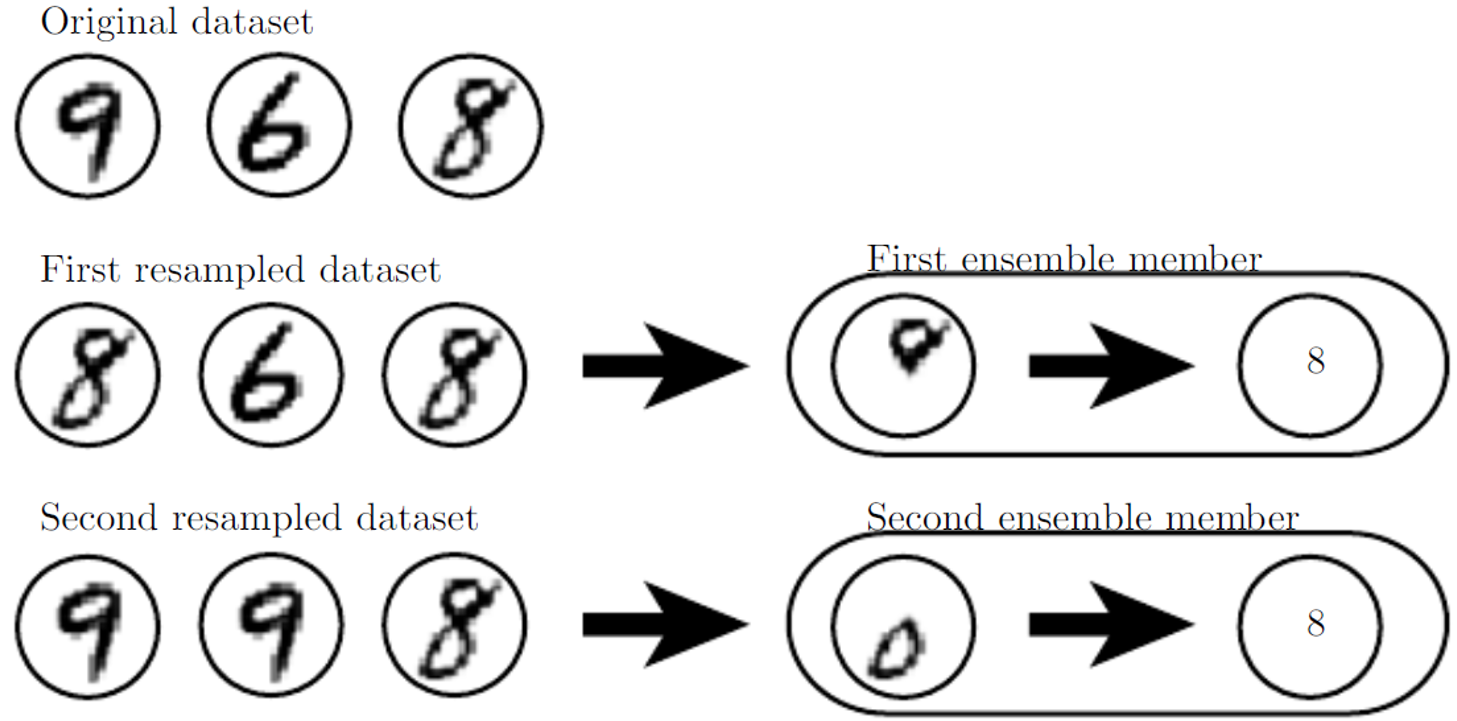
\includegraphics[width=0.85\linewidth]{images/bagging.PNG}
	\end{figure}
	Differences in random initialization, random selection of minibatches, differences in hyperparameters, or different outcomes of non-deterministic implementations of neural networks are often enough to cause different members of the ensemble to make partially independent errors.

	\subsection{Noise Robustness \& Dropout}
	Dropout provides a computationally inexpensive but powerful method of regularizing a broad family of models.
	Dropout can be thought of as a method of making bagging practical for ensembles of very many large neural networks.
	Bagging involves training multiple models, and evaluating multiple models on each test example.
	This seems \textbf{impractical} when each model is a \textbf{large neural network}, since training and evaluating such networks is \textbf{costly in terms of runtime and memory}.\\

	Dropout trains the ensemble consisting of all sub-networks that can be formed by \textbf{removing non-output units} from an underlying base network.
	In the example below, there are 4 non-output units, each can either be part of the network or not. Hence there are $2^4=16$ possible configurations.
	\begin{figure}[H]
		\centering
		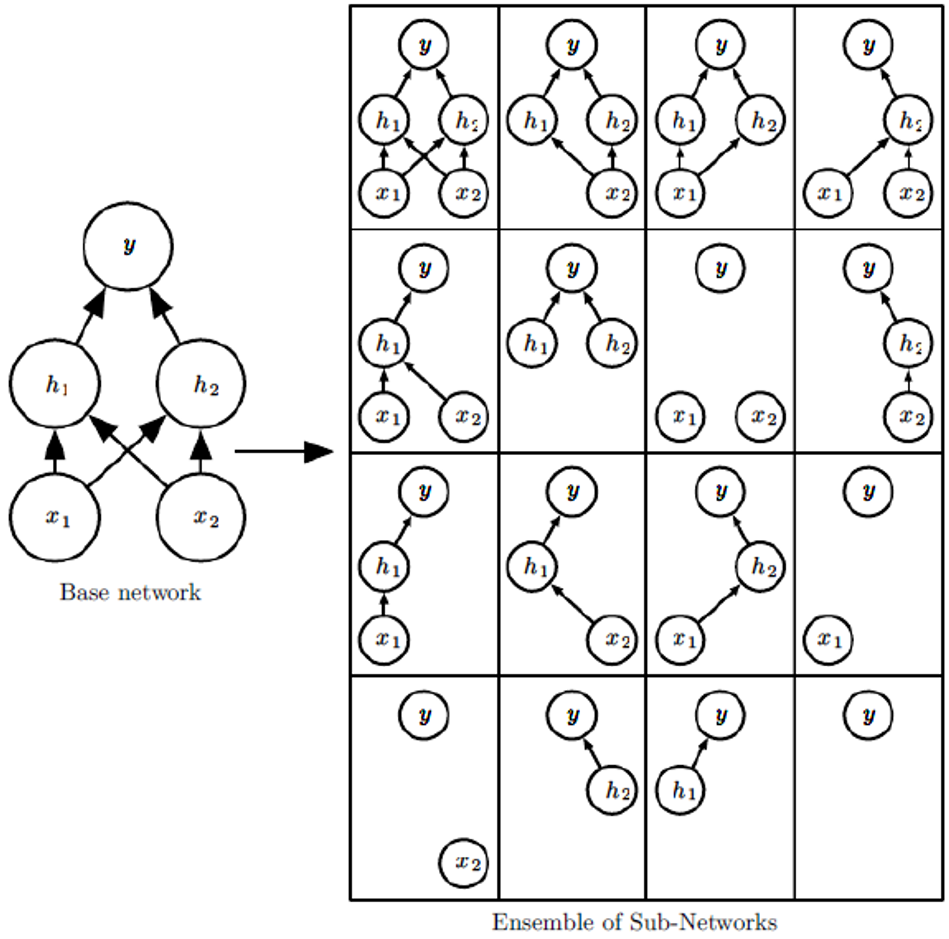
\includegraphics[width=0.9\linewidth]{images/dropoutensemble.png}
	\end{figure}
	In most modern neural networks, based on a series of affine transformations and nonlinearities, we can effectively remove a unit from a network by \textbf{multiplying its output value by zero}.
	Each time we load an example into a minibatch, we randomly sample a different binary mask to apply to all of the input and hidden units in the network. The mask for each unit is sampled independently from all of the others.\\

	The \textbf{probability of sampling a mask value} of one (causing a unit to be included) is a \textbf{hyperparameter fixed before training begins}. It is not a function of the current value of the model parameters or the input example.
	Typically, an input unit is included with probability 0.8 and a hidden unit is included with probability 0.5. We then run forward propagation, back-propagation, and the learning update as usual.\\

	In the case of bagging, the models are all independent. In the case of dropout, the models \textbf{share parameters}, with each model inheriting a different subset of parameters from the parent neural network.
	This parameter sharing makes it possible to represent an exponential number of models with a tractable amount of memory.\\

	In the case of bagging, each model is trained to convergence on its respective training set.
	In the case of dropout, typically most models are not explicitly trained at all—usually, the model is large enough that it would be infeasible to sample all possible subnetworks. Instead, a tiny fraction of the possible sub-networks are each trained for a single step (minibatch), and the parameter sharing causes the remaining sub-networks to arrive at good settings of the parameters.\\

	These are the only differences. Beyond these, dropout follows the bagging algorithm. For example, the training set encountered by each sub-network is indeed a subset of the original training set sampled with replacement, i.e., a minibatch.\\

	Now, we assume that the model's role is to output a probability distribution.
	In the case of bagging, each model $i$ produces a probability distribution $ p^{(i)}(y|\vx) $.
	The prediction of the ensemble is given by the arithmetic mean of all of these distributions:
	\[ \frac{1}{k}\sum_{i=1}^{k}p^{(i)}(y|\vx) \]
	In the case of dropout, each sub-model defined by mask vector $\vmu$ defines a probability distribution.
	The arithmetic mean over all masks is given by
	\[ \sum_\vmu p(\vmu)p(y|\vx,\vmu) \]
	where $p(\vmu)$ is the probability distribution that was used to sample $\vmu$ at training time.

	There is plenty of evidence that the \textbf{geometric mean} performs comparably to the arithmetic mean in this context.
	To guarantee that the result is a probability distribution, we impose the requirement that none of the sub-models assigns probability 0 to any event, and we re-normalize the resulting distribution.
	The unnormalized probability distribution defined directly by the geometric mean is given by
	\[ \tilde{p}_{\text{ensemble}}(y|\vx) = \sqrt[2^d]{\prod_\vmu p(y|\vx,\vmu)} \]

	To make predictions we must re-normalize the ensemble:
	\[ p_{\text{ensemble}}(y|\vx) = \frac{\tilde{p}_{\text{ensemble}}(y|\vx)}{\sum_{y'}\tilde{p}_{\text{ensemble}}(y'|\vx)} \]
	Amazingly, we can approximate this distribution $p_{\text{ensemble}}(y|\vx)$ by evaluating $p(y|\vx)$ in \textbf{one} model.
	The motivation for this modification is to capture the right expected value of the output from that unit.
	Because we usually use an inclusion probability of 0.5, this rule basically amounts to \textbf{dividing the weights by 2} at the end of training, and then using the model as usual.
	The goal is to make sure that the expected total input to a unit at test time is roughly the same as the expected total input to that unit at train time, even though half the units at train time are missing on average.\\

	For many classes of models that do not have nonlinear hidden units, this rule is exact.
	For a simple example, consider a softmax regression classifier with $n$ input variables represented by the $n$-dimensional vector $\vv$:
	\[ P(\ry=y|\vv) =\softmax\left(\mW^T\vv+\vb\right)_y \]

	We can index into the family of sub-models by element-wise multiplication of the input with a binary vector $\vd$:
	\[ P(\ry=y|\vv;\vd) = \softmax\left(\mW^T(\vd\odot\vv)+\vb\right)_y \]

	The ensemble predictor is defined by re-normalizing the geometric mean over all ensemble members predictions
	\[ \tilde{P}_{\text{ensemble}}(\ry=y|\vv) = \sqrt[2^n]{\prod_{\vd\in\{0,1\}^n} P(\ry=y|\vv;\vd)} \]

	Again, the assumption is, that each element of the vector $\vd$ has a probability of 0.5 to be either 0 or 1. Hence this uniform distribution simplifies the presentation, since $p(\vd)$ is a constant and hence will cancel out
	\[ P_{\text{ensemble}}(\ry=y|\vv) = \frac{\tilde{P}_{\text{ensemble}}(\ry=y|\vv)} {\sum_{y'}\tilde{P}_{\text{ensemble}}(\ry=y'|\vv)} \]

	\textbf{Dropout is computationally cheap}: Using dropout during training requires only $O(n)$ computation per example per update, to generate $n$ random binary numbers and multiply them by the state.
	Running inference in the trained model has the same cost per-example as if dropout were not used, though we must pay the cost of dividing the weights by 2 once before beginning to run inference on examples.\\

	For very large datasets, regularization confers little reduction in generalization error.
	In these cases, the computational cost of using dropout and larger models may outweigh the benefit of regularization.\\

	The \textbf{power of dropout} arises from the fact that the masking noise is applied to the hidden units.
	This can be seen as a form of highly intelligent, adaptive destruction of the information content of the input rather than destruction of the raw values of the input.\\
	For \textbf{example}, if the model learns a hidden unit that detects a face by finding the nose, then dropping this unit corresponds to erasing the information that there is a nose in the image.
	The model must learn another hidden unit, either that redundantly encodes the presence of a nose, or that detects the face by another feature, such as the mouth.
	Destroying extracted features rather than original values allows the destruction process to make use of all of the knowledge about the input distribution that the model has acquired so far.

%	\subsection{Bagging and other Ensemble Methods}
%	The idea is to train several different models separately, then have all of the models vote on the output for test examples.
%	This is an example of a general strategy in machine learning called model averaging. Techniques employing this strategy are known as \textbf{ensemble methods}.
%	The main reason why this works is, that different models will make different, and \emph{ideally, uncorrelated}, errors. Hence averaging the model responses will reduce the variance of the errors:
%	\begin{align*}
%	\E\left[\left(\frac{1}{k}\sum_i\epsilon_i\right)^2\right]
%	&= \frac{1}{k^2}\E\left[\sum_i\left(\epsilon_i^2+\sum_{j\neq i}\epsilon_i\epsilon_j\right)\right]\\
%	&= \frac{1}{k}v+\frac{k-1}{k}c
%	\end{align*}
%	The formula clearly shows, that for perfectly correlated errors $(c=v)$, averaging the predictions and hence averaging the errors does not help.
%	In the case the errors are completely \textbf{uncorrelated} $c=0$, the well known result is achieved, that the error variance $v$ is reduced by the number of models $k$.
%	Hence in the \textbf{worst case} it is not worse than a single model.
%	In the \textbf{best case} it is better by a factor $k$. This assumes that the mean error is zero.\\
%
%	\textbf{Bootstrap aggregating (bagging)} is a method that allows the same kind of model, training algorithm and objective function to be reused several times.
%	Bagging involves constructing $k$ different datasets. Each dataset has the same number of examples as the original dataset, but each dataset is constructed by sampling with replacement from the original dataset.\\
%	This means that, with high probability, each dataset is missing some of the examples from the original dataset and also contains several duplicate examples (on average around $2/3$ of the examples from the original dataset are found in the resulting training set, if it has the same size as the original).\\
%	Model $i$ is then trained on dataset $i$. The differences between which examples are included in each dataset result in differences between the trained models.
%	\begin{figure}[H]
%		\centering
%		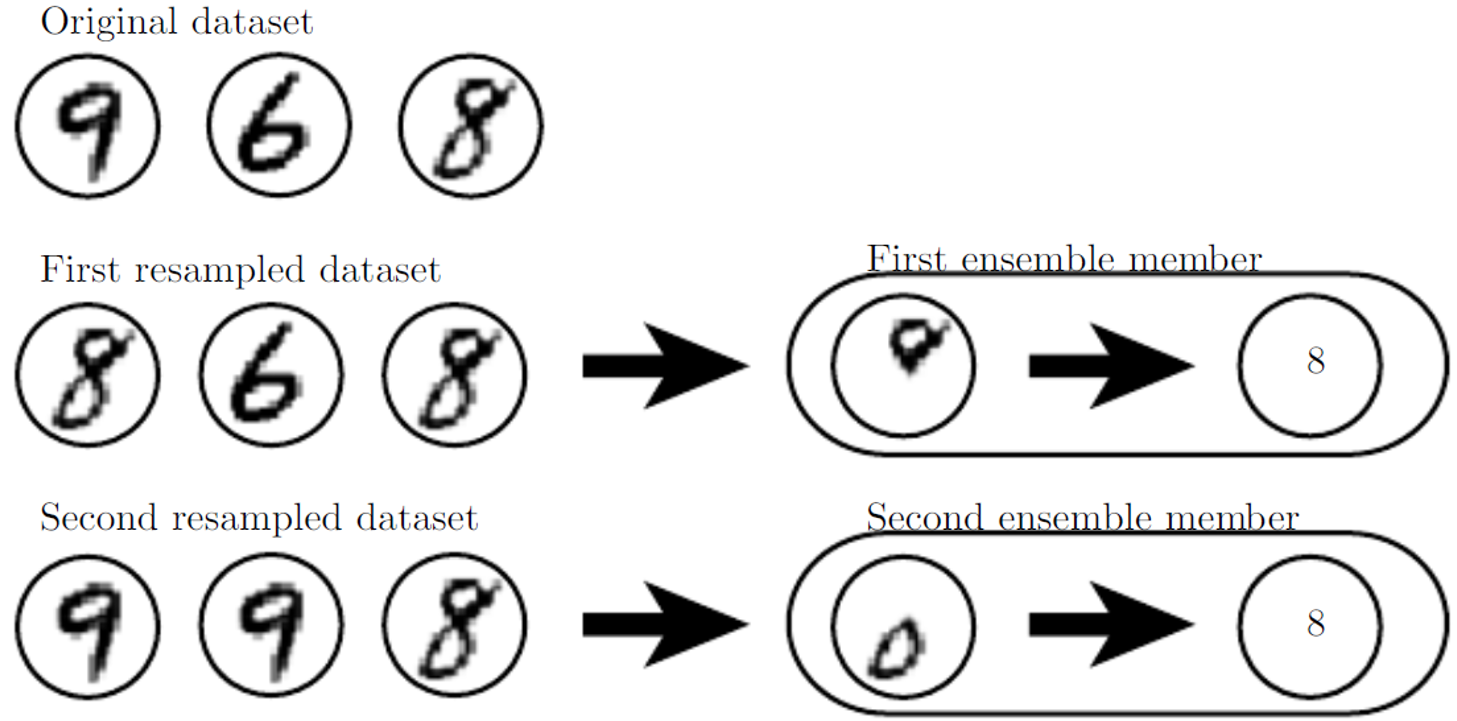
\includegraphics[width=0.85\linewidth]{images/bagging.PNG}
%	\end{figure}
%	Differences in random initialization, random selection of minibatches, differences in hyperparameters, or different outcomes of non-deterministic implementations of neural networks are often enough to cause different members of the ensemble to make partially independent errors.
%
%	\subsection{Dropout}
%	Dropout provides a computationally inexpensive but powerful method of regularizing a broad family of models.
%	Dropout can be thought of as a method of making bagging practical for ensembles of very many large neural networks.
%	Bagging involves training multiple models, and evaluating multiple models on each test example.
%	This seems \textbf{impractical} when each model is a \textbf{large neural network}, since training and evaluating such networks is \textbf{costly in terms of runtime and memory}.\\
%
%	Dropout trains the ensemble consisting of all sub-networks that can be formed by \textbf{removing non-output units} from an underlying base network.
%	In the example below, there are 4 non-output units, each can either be part of the network or not. Hence there are $2^4=16$ possible configurations.
%	\begin{figure}[H]
%		\centering
%		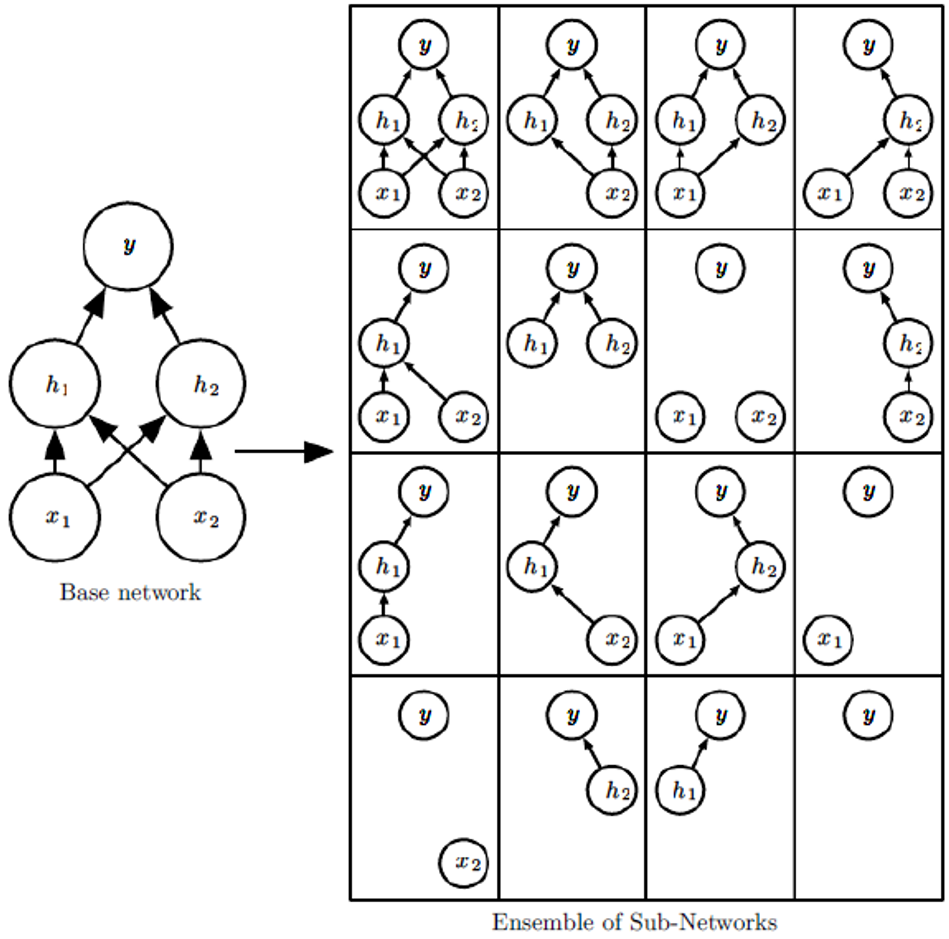
\includegraphics[width=0.9\linewidth]{images/dropoutensemble.png}
%	\end{figure}
%	In most modern neural networks, based on a series of affine transformations and nonlinearities, we can effectively remove a unit from a network by \textbf{multiplying its output value by zero}.
%	Each time we load an example into a minibatch, we randomly sample a different binary mask to apply to all of the input and hidden units in the network. The mask for each unit is sampled independently from all of the others.\\
%
%	The \textbf{probability of sampling a mask value} of one (causing a unit to be included) is a \textbf{hyperparameter fixed before training begins}. It is not a function of the current value of the model parameters or the input example.
%	Typically, an input unit is included with probability 0.8 and a hidden unit is included with probability 0.5. We then run forward propagation, back-propagation, and the learning update as usual.\\
%
%	In the case of bagging, the models are all independent. In the case of dropout, the models \textbf{share parameters}, with each model inheriting a different subset of parameters from the parent neural network.
%	This parameter sharing makes it possible to represent an exponential number of models with a tractable amount of memory.\\
%
%	In the case of bagging, each model is trained to convergence on its respective training set.
%	In the case of dropout, typically most models are not explicitly trained at all—usually, the model is large enough that it would be infeasible to sample all possible subnetworks. Instead, a tiny fraction of the possible sub-networks are each trained for a single step (minibatch), and the parameter sharing causes the remaining sub-networks to arrive at good settings of the parameters.\\
%
%	These are the only differences. Beyond these, dropout follows the bagging algorithm. For example, the training set encountered by each sub-network is indeed a subset of the original training set sampled with replacement, i.e., a minibatch.\\
%
%	Now, we assume that the models role is to output a probability distribution.
%	In the case of bagging, each model $i$ produces a probability distribution
%	The prediction of the ensemble is given by the arithmetic mean of all of these distributions:
%	\[ \frac{1}{k}\sum_{i=1}^{k}p^{(i)}(y|\vx) \]
%	In the case of dropout, each sub-model defined by mask vector $\vmu$ defines a probability distribution.
%	The arithmetic mean over all masks is given by
%	\[ \sum_\vmu p(\vmu)P(y|\vx,\vmu) \]
%	where $p(\vmu)$ is the probability distribution that was used to sample $\vmu$ at training time.
%
%	There is plenty of evidence that the \textbf{geometric mean} performs comparably to the arithmetic mean in this context.
%	To guarantee that the result is a probability distribution, we impose the requirement that none of the sub-models assigns probability 0 to any event, and we renormalize the resulting distribution.
%	The unnormalized probability distribution defined directly by the geometric mean is given by
%	\[ \tilde{p}_{\text{ensemble}}(y|\vx) = \sqrt[2^d]{\prod_\vmu p(y|\vx,\vmu)} \]
%
%	To make predictions we must re-normalize the ensemble:
%	\[ p_{\text{ensemble}}(y|\vx) = \frac{\tilde{p}_{\text{ensemble}}(y|\vx)}{\sum_{y'}\tilde{p}_{\text{ensemble}}(y'|\vx)} \]
%	Amazingly we can approximate this distribution $p_{\text{ensemble}}(y|\vx)$ by evaluating $p(y|\vx)$ in \textbf{one} model.
%	The motivation for this modification is to capture the right expected value of the output from that unit.
%	Because we usually use an inclusion probability of 0.5, this rule basically amounts to \textbf{dividing the weights by 2} at the end of training, and then using the model as usual.
%	The goal is to make sure that the expected total input to a unit at test time is roughly the same as the expected total input to that unit at train time, even though half the units at train time are missing on average.\\
%
%	For many classes of models that do not have nonlinear hidden units, this rule is exact.
%	For a simple example, consider a softmax regression classifier with $n$ input variables represented by the $n$-dimensional vector $\vv$:
%	\[ P(\ry=y|\vv) =\softmax\left(\mW^T\vv+\vb\right)_y \]
%
%	We can index into the family of sub-models by element-wise multiplication of the input with a binary vector $\vd$:
%	\[ P(\ry=y|\vv;\vd) = \softmax\left(\mW^T(\vd\odot\vv)+\vb\right)_y \]
%
%	The ensemble predictor is defined by re-normalizing the geometric mean over all ensemble members predictions
%	\[ \tilde{P}_{\text{ensemble}}(\ry=y|\vv) = \sqrt[2^n]{\prod_{\vd\in\{0,1\}^n} P(\ry=y|\vv;\vd)} \]
%
%	Again, the assumption is, that each element of the vector $\vd$ has a probability of 0.5 to be either 0 or 1. Hence this uniform distribution simplifies the presentation, since $p(\vd)$ is a constant and hence will cancel out
%	\[ P_{\text{ensemble}}(\ry=y|\vv) = \frac{\tilde{P}_{\text{ensemble}}(\ry=y|\vv)} {\sum_{y'}\tilde{P}_{\text{ensemble}}(\ry=y'|\vv)} \]
%
%	\textbf{Dropout is computationally cheap}: Using dropout during training requires only $O(n)$ computation per example per update, to generate $n$ random binary numbers and multiply them by the state.
%	Running inference in the trained model has the same cost per-example as if dropout were not used, though we must pay the cost of dividing the weights by 2 once before beginning to run inference on examples.\\
%
%	For very large datasets, regularization confers little reduction in generalization error.
%	In these cases, the computational cost of using dropout and larger models may outweigh the benefit of regularization.\\
%
%	The \textbf{power of dropout} arises from the fact that the masking noise is applied to the hidden units.
%	This can be seen as a form of highly intelligent, adaptive destruction of the information content of the input rather than destruction of the raw values of the input.\\
%	For \textbf{example}, if the model learns a hidden unit that detects a face by finding the nose, then dropping this unit corresponds to erasing the information that there is a nose in the image.
%	The model must learn another hidden unit, either that redundantly encodes the presence of a nose, or that detects the face by another feature, such as the mouth.
%	Destroying extracted features rather than original values allows the destruction process to make use of all of the knowledge about the input distribution that the model has acquired so far.

\end{multicols}
\newpage
